\documentclass{article}
\usepackage{amsmath, amsthm, amsfonts, amssymb}
\usepackage{cite} 
\usepackage{float}
\usepackage{enumitem}
\usepackage[margin=10pt,font=small,labelfont=bf]{caption}
\usepackage{graphicx}
\graphicspath{ {./} }

\renewcommand{\figurename}{Slika}

\DeclareMathOperator{\mse}{MSE}
\DeclareMathOperator{\var}{var}
\DeclareMathOperator{\Var}{Var}
\DeclareMathOperator{\se}{SE}
\DeclareMathOperator{\ci}{CI}

\title{Projektna naloga iz Statistike}
\author{David Čadež}
\date{}

\begin{document}

\maketitle

\section{Prva naloga}

Pri prvi nalogi bomo obravnavali izobrazbo $43.866$ družin, ki stanujejo v mestu
Kibergrad. Pomagali si bomo z enostavnim vzorčenjem in ocenjevali delež družin,
v katerih vodja gospodinjstva nima srednješolske izobrazbe.

Najprej definiramo novo spremenljivko $Y$, ki je indikator dogodka \emph{vodja
gospodinjstva nima srednješolske izobrazbe}. Delež gospodinjstev, v katerih
vodja nima srednješolske izobrazbe je v tem primeru povprečje spremenljivke $Y$
na populaciji.

Pomagal sem si s programom \textbf{naloga1.py}. Če ga poženemo, vrne spodnji
izhod.
\begin{verbatim}
a) Ocena za delež je 0.200.
b) Ocena za standardno napako je 0.02829,
interval zaupanja pa je (0.14455, 0.25545).
c) Da, interval zaupanja pokrije populacijski delež: 0.21150
Prava standardna napaka je enaka 0.02888.
d) Pri n=200 92.0% intervalov zaupanja pokrije populacijski delež.
e) Standardni odklon vzorčnih deležev za n=200 je 0.02902,
prava standardna napaka za vzorec velikosti 200 pa 0.02888
f) Pri n=800 98.0% intervalov zaupanja pokrije populacijski delež.
Standardni odklon vzorčnih deležev za n=800 je 0.01209,
prava standardna napaka za vzorec velikosti 800 pa 0.01431
\end{verbatim}


\begin{enumerate}[label=\alph*)]
    \item Pri prvi podnalogi vzamemo slučajen vzorec velikosti $200$. Ker želimo
        oceniti pričakovano vrednost na populaciji, za cenilko vzamemo enostavno
        povprečje na vzorcu. S programom \textbf{naloga1.py} sem dobil oceno za
        delež $\hat{d} = 0{,}200$.
    \item Standardno napako ocenimo z nepristransko cenilko
        \[
            \widehat{\se}_+^2 = \frac{N - n}{N n} \frac{\sum_{i=1}^{n} (x_i -
            \bar{x})^2}{n - 1}
        \]
        Program \textbf{naloga1.py} na podlagi vzorca vrne približek
        $0{,}02829$. Z uporabo te ocene za standardno napako lahko izračunamo
        interval zaupanja kot
        \[
            \ci = (\hat{d} - 1{,}96 \widehat{\se}_+^2, \hat{d} + 1{,}96
            \widehat{\se}_+^2).
        \]
        Program \textbf{naloga1.py} vrne interval zaupanja $(0.14455, 0.25545)$.
    \item Pravi delež ljudi, ki nimajo srednješolske izobrazbe je približno
        $0{,}21150$, torej zgornji interval zaupanja pokrije populacijski delež.
        Prava standardna napaka pa je približno $0{,}02888$.
    \item Vzemimo sedaj še $99$ novih enostavnih slučajnih vzorcev in pri vsakem
        določimo interval zaupanja. Na sliki~\ref{slika 1d} so narisani ti
        intervali zaupanja. Program izračuna, da jih $92$ \% pokrije
        populacijsko povprečje, kar je blizu $95$ \%.
        \begin{figure}[H]
            \centering
            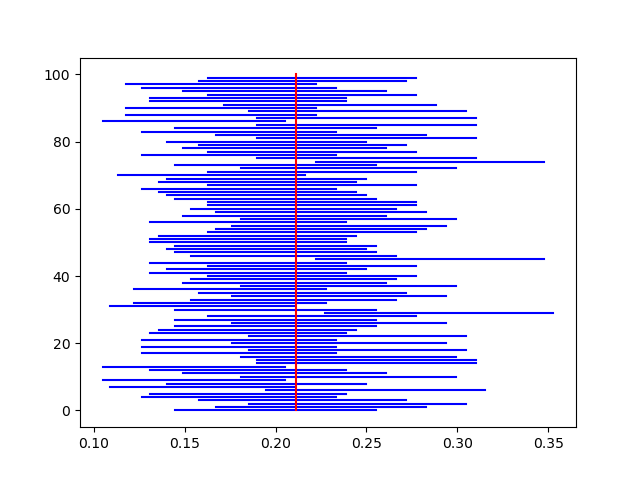
\includegraphics[scale=0.5]{1d.png}
            \label{slika 1d}
            \caption{Intervali zaupanja za $100$ enostavnih slučajnih vzorcev
            velikosti $200$. Z rdečo je označeno populacijsko povprečje.}
        \end{figure}
    \item Standardni odklon vzorčnih deležev je približno $0{,}02902$, kar je
        približno enako kot standardna napaka za vzorec velikosti $200$.
    \item Sedaj pa izvedimo podobno še na $100$ vzorcih velikosti $800$. Na
        sliki~\ref{slika 1f} vidimo, da so intervali v povprečju ožji kot na
        sliki~\ref{slika 1d}. To je zato, ker je standardni odklon vzorčnih
        deležev manjši, če vzamemo večje deleže. Standardni odklon vzorčnih
        deležev teh $100$ vzorcev velikosti $800$ je približno $0{,}01209$.
        Torej je res manjši od iste vrednosti za manjše vzorce. Prava standardna
        napaka za vzorec velikosti pa je enaka $0{,}01431$. Če bi vzeli več
        vzorcev, bi bil standardni odklon vzorčnih deležev v povprečju bližje
        pravi standardni napaki za vzorec te velikosti.
        \begin{figure}[H]
            \centering
            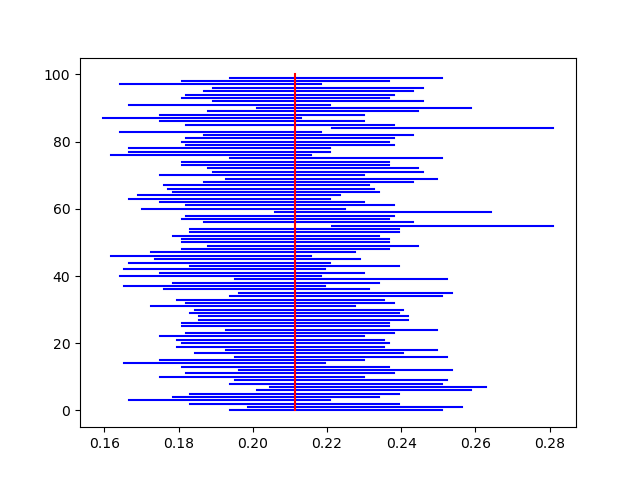
\includegraphics[scale=0.5]{1f.png}
            \label{slika 1f}
            \caption{Intervali zaupanja za $100$ enostavnih slučajnih vzorcev
            velikosti $800$. Z rdečo je označeno populacijsko povprečje.}
        \end{figure}
\end{enumerate}

\section{Druga naloga}

Opazujemo normalnost 
\begin{figure}[H]
    \caption{}
    \centering
    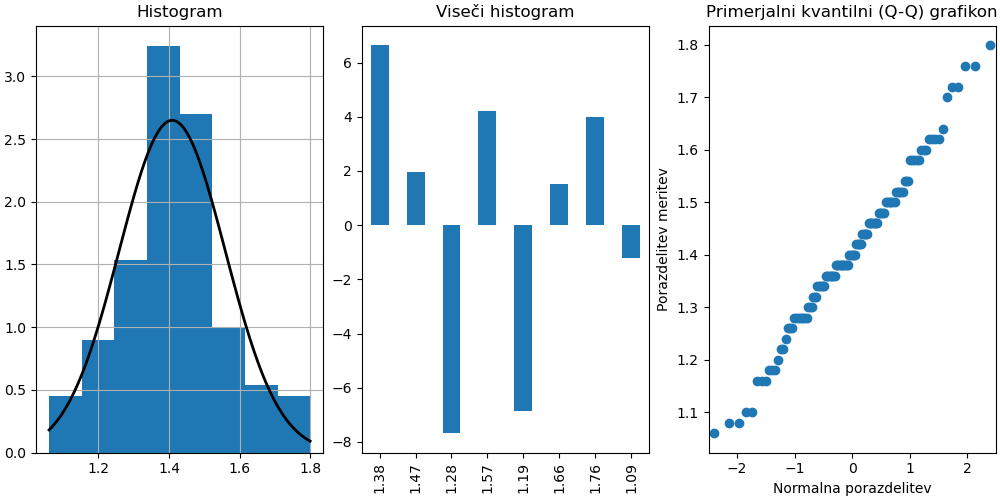
\includegraphics[scale=0.5]{2.png}
\end{figure}

\section{Tretja naloga}

\nocite{*}
\bibliographystyle{siam}
\bibliography{viri}{}

\end{document}
